\documentclass[11pt,a4paper]{report}
\usepackage[textwidth=37em,vmargin=30mm]{geometry}
\usepackage{calc,xunicode,amsmath,amssymb,paralist,enumitem,tabu,booktabs,datetime2,xeCJK,xeCJKfntef,listings}
\usepackage{tocloft,fancyhdr,tcolorbox,xcolor,graphicx,eso-pic,xltxtra,xelatexemoji}

\newcommand{\envyear}[0]{2024}
\newcommand{\envdatestr}[0]{2024-11-05}
\newcommand{\envfinaldir}[0]{webdb/2024/20241105/final}

\usepackage[hidelinks]{hyperref}
\hypersetup{
    colorlinks=false,
    pdfpagemode=FullScreen,
    pdftitle={Web Digest - \envdatestr}
}

\setlength{\cftbeforechapskip}{10pt}
\renewcommand{\cftchapfont}{\rmfamily\bfseries\large\raggedright}
\setlength{\cftbeforesecskip}{2pt}
\renewcommand{\cftsecfont}{\sffamily\small\raggedright}

\setdefaultleftmargin{2em}{2em}{1em}{1em}{1em}{1em}

\usepackage{xeCJK,xeCJKfntef}
\xeCJKsetup{PunctStyle=plain,RubberPunctSkip=false,CJKglue=\strut\hskip 0pt plus 0.1em minus 0.05em,CJKecglue=\strut\hskip 0.22em plus 0.2em}
\XeTeXlinebreaklocale "zh"
\XeTeXlinebreakskip = 0pt


\setmainfont{Brygada 1918}
\setromanfont{Brygada 1918}
\setsansfont{IBM Plex Sans}
\setmonofont{JetBrains Mono NL}
\setCJKmainfont{Noto Serif CJK SC}
\setCJKromanfont{Noto Serif CJK SC}
\setCJKsansfont{Noto Sans CJK SC}
\setCJKmonofont{Noto Sans CJK SC}

\setlength{\parindent}{0pt}
\setlength{\parskip}{8pt}
\linespread{1.15}

\lstset{
	basicstyle=\ttfamily\footnotesize,
	numbersep=5pt,
	backgroundcolor=\color{black!5},
	showspaces=false,
	showstringspaces=false,
	showtabs=false,
	tabsize=2,
	captionpos=b,
	breaklines=true,
	breakatwhitespace=true,
	breakautoindent=true,
	linewidth=\textwidth
}






\newcommand{\coverpic}[2]{
    % argv: itemurl, authorname
    Cover photo by #2~~(\href{#1}{#1})
}
\newcommand{\makeheader}[0]{
    \begin{titlepage}
        % \newgeometry{hmargin=15mm,tmargin=21mm,bmargin=12mm}
        \begin{center}
            
            \rmfamily\scshape
            \fontspec{BaskervilleF}
            \fontspec{Old Standard}
            \fontsize{59pt}{70pt}\selectfont
            WEB\hfill DIGEST
            
            \vfill
            % \vskip 30pt
            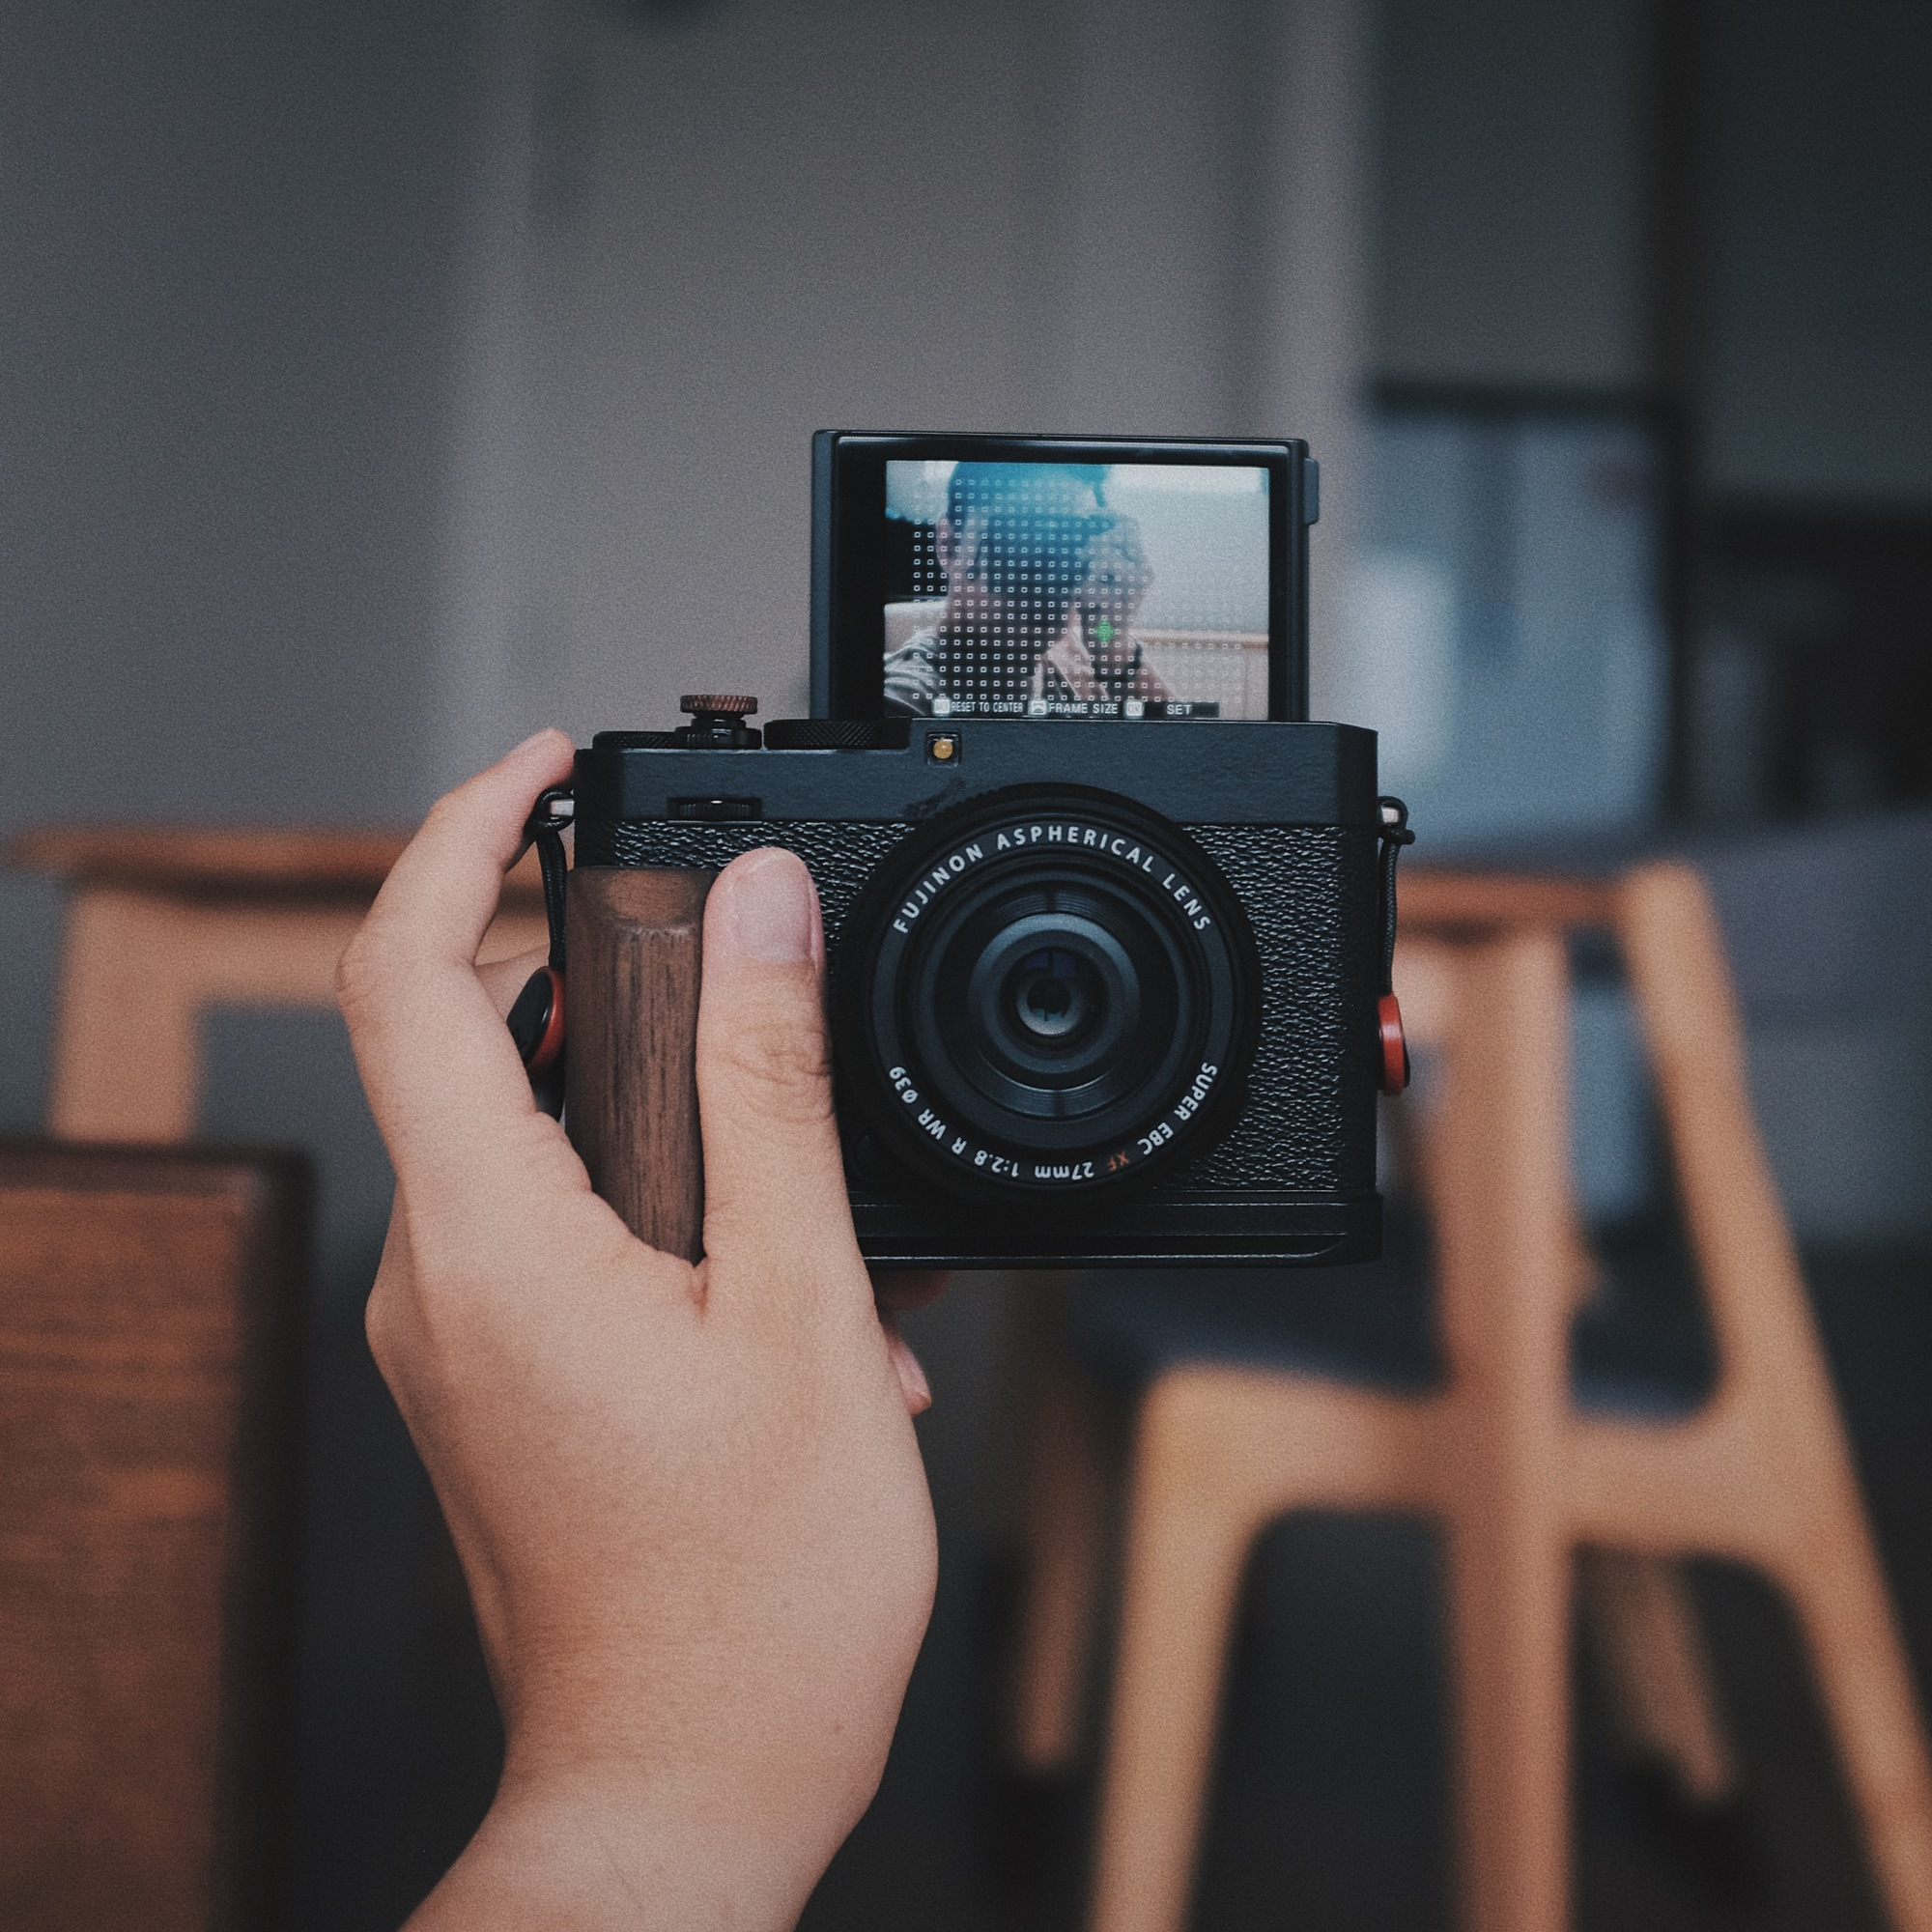
\includegraphics[width=\linewidth]{\envfinaldir/coverpic-prod.jpg}\par
            % \vskip 30pt
            \vfill

            \normalsize\rmfamily\scshape
            \copyright{} The Web Digest Project \hfill\large \envdatestr
        \end{center}
    \end{titlepage}
    % \restoregeometry
}
\newcommand{\simplehref}[1]{%
    \textcolor{blue!80!green}{\href{#1}{#1}}%
}
\renewcommand{\contentsname}{\center\Huge\sffamily\bfseries Contents\par\vskip 20pt}
\newcounter{ipartcounter}
\setcounter{ipartcounter}{0}
\newcommand{\ipart}[1]{
    % \vskip 20pt
    \clearpage
    \stepcounter{ipartcounter}
    \phantomsection
    \addcontentsline{toc}{chapter}{#1}
    % \begin{center}
    %     \Huge
    %     \sffamily\bfseries
    %     #1
    % \end{center}
    % \vskip 20pt plus 7pt
}
\newcounter{ichaptercounter}
\setcounter{ichaptercounter}{0}
\newcommand{\ichapter}[1]{
    % \vskip 20pt
    \clearpage
    \stepcounter{ichaptercounter}
    \phantomsection
    \addcontentsline{toc}{section}{\numberline{\arabic{ichaptercounter}}#1}
    \begin{center}
        \Huge
        \sffamily\bfseries
        #1
    \end{center}
    \vskip 20pt plus 7pt
}
\newcommand{\entrytitlefont}[1]{\subsection*{\raggedright\Large\sffamily\bfseries#1}}
\newcommand{\entryitemGeneric}[2]{
    % argv: title, url
    \parbox{\linewidth}{
        \entrytitlefont{#1}\par\vskip 5pt
        \footnotesize\ttfamily\mdseries
        \simplehref{#2}
    }\vskip 11pt plus 11pt minus 1pt
}
\newcommand{\entryitemGithub}[3]{
    % argv: title, url, desc
    \parbox{\linewidth}{
        \entrytitlefont{#1}\par\vskip 5pt
        \footnotesize\ttfamily\mdseries
        \simplehref{#2}\par\vskip 5pt
        \small\rmfamily\mdseries#3
    }\vskip 11pt plus 11pt minus 1pt
}
\newcommand{\entryitemAp}[3]{
    % argv: title, url, desc
    \parbox{\linewidth}{
        \entrytitlefont{#1}\par\vskip 5pt
        \footnotesize\ttfamily\mdseries
        \simplehref{#2}\par\vskip 5pt
        \small\rmfamily\mdseries#3
    }\vskip 11pt plus 11pt minus 1pt
}
\newcommand{\entryitemHackernews}[3]{
    % argv: title, hnurl, rawurl
    % \parbox{\linewidth}{
    %     \entrytitlefont{#1}\par\vskip 5pt
    %     \footnotesize\ttfamily\mdseries
    %     \simplehref{#3}\par
    %     \textcolor{black!50}{\href{#2}{#2}}
    % }\vskip 11pt plus 11pt minus 1pt
    \begin{minipage}{\linewidth}
            \entrytitlefont{#1}\par\vskip 5pt
            \footnotesize\ttfamily\mdseries
            \simplehref{#3}\par
            \textcolor{black!50}{\href{#2}{#2}}
    \end{minipage}\par\vskip 11pt plus 11pt minus 1pt
}







\begin{document}

\makeheader

\tableofcontents\clearpage




\ipart{Developers}
\ichapter{Hacker News}
\entryitemTwoLinks{Albertsons kills rural grocers with land use restrictions}{https://news.ycombinator.com/item?id=42046196}{https://www.thebignewsletter.com/p/how-albertsons-kills-rural-grocers}

\entryitemTwoLinks{Writing secure Go code}{https://news.ycombinator.com/item?id=42043939}{https://jarosz.dev/article/writing-secure-go-code/}

\entryitemTwoLinks{We're Leaving Kubernetes}{https://news.ycombinator.com/item?id=42041917}{https://www.gitpod.io/blog/we-are-leaving-kubernetes}

\entryitemTwoLinks{New York Times Tech Guild goes on strike}{https://news.ycombinator.com/item?id=42040795}{https://www.washingtonpost.com/style/media/2024/11/04/new-york-times-tech-strike-walkout/}

\entryitemTwoLinks{Is the Q source the origin of the Gospels?}{https://news.ycombinator.com/item?id=42040706}{https://www.thecollector.com/q-source-origin-gospels/}

\entryitemTwoLinks{A change of heart regarding employee metrics}{https://news.ycombinator.com/item?id=42038653}{http://rachelbythebay.com/w/2024/11/03/metrics/}

\entryitemTwoLinks{Please just stop saying "just" (2019)}{https://news.ycombinator.com/item?id=42038139}{https://sgringwe.com/2019/10/10/Please-just-stop-saying-just.html}

\entryitemTwoLinks{An embarrassingly simple approach to recover unlearned knowledge for LLMs}{https://news.ycombinator.com/item?id=42037982}{https://arxiv.org/abs/2410.16454}

\entryitemTwoLinks{Scientists glue two proteins together, driving cancer cells to self-destruct}{https://news.ycombinator.com/item?id=42037386}{https://med.stanford.edu/news/all-news/2024/10/protein-cancer.html}

\entryitemTwoLinks{Why systemd is a problem for embedded Linux}{https://news.ycombinator.com/item?id=42036305}{https://kevinboone.me/systemd\_embedded.html}

\entryitemTwoLinks{Do you need Redis? PostgreSQL does queuing, locking, and pub/sub (2021)}{https://news.ycombinator.com/item?id=42036303}{https://spin.atomicobject.com/redis-postgresql/}

\entryitemTwoLinks{Show HN: Tinder, but to decide what to eat}{https://news.ycombinator.com/item?id=42036041}{https://whatdinner.com/}

\entryitemTwoLinks{Project Sid: Many-agent simulations toward AI civilization}{https://news.ycombinator.com/item?id=42035319}{https://github.com/altera-al/project-sid}

\entryitemTwoLinks{I couldn't find a free, no-login, no-AI checklist app–so I built one}{https://news.ycombinator.com/item?id=42034146}{https://lalacheck.fly.dev/}

\entryitemTwoLinks{Touchscreens are out, and tactile controls are back}{https://news.ycombinator.com/item?id=42033241}{https://spectrum.ieee.org/touchscreens}

\entryitemTwoLinks{Intel might be too big to fail}{https://news.ycombinator.com/item?id=42032906}{https://www.tomshardware.com/tech-industry/intel-might-be-too-big-to-fail-washington-policymakers-are-already-discussing-potential-solutions-if-the-chipmaker-cannot-recover}

\entryitemTwoLinks{If you need the money, don't take the job}{https://news.ycombinator.com/item?id=42032638}{https://bitfieldconsulting.com/posts/need-money}

\entryitemTwoLinks{Matrix 2.0 Is Here}{https://news.ycombinator.com/item?id=42032387}{https://matrix.org/blog/2024/10/29/matrix-2.0-is-here/?resubmit}

\entryitemTwoLinks{Ask HN: What would you preserve if the internet were to go down tomorrow?}{https://news.ycombinator.com/item?id=42030832}{https://news.ycombinator.com/item?id=42030832}

\entryitemTwoLinks{Security flaws found in Nvidia GeForce GPUs}{https://news.ycombinator.com/item?id=42030463}{https://www.pcworld.com/article/2504035/security-flaws-found-in-all-nvidia-geforce-gpus-update-drivers-asap.html}\ichapter{Phoronix}
\entryitemGeneric{\hskip 0pt{}Intel Releases x86-simd-sort 6.0 For Speedy AVX2/AVX-512 Sorting, PyTorch Now Using It}{https://www.phoronix.com/news/x86-simd-sort-6.0}

\entryitemGeneric{\hskip 0pt{}Linux Preps New AMD ERAPS Feature With EPYC Turin To Benefit Performance}{https://www.phoronix.com/news/AMD-ERAPS-Linux}

\entryitemGeneric{\hskip 0pt{}TOUPUWAN 30-Slot Laptop/Tablet Storage Cart}{https://www.phoronix.com/review/toupuwan-30-32-laptop-cart}

\entryitemGeneric{\hskip 0pt{}Manjaro Linux Working On "Manjaro Data Donor" As New Data Collection Tool}{https://www.phoronix.com/news/Manjaro-Linux-Data-Donor}

\entryitemGeneric{\hskip 0pt{}Fujitsu Monaka CPU Target Added To GCC 15 Compiler}{https://www.phoronix.com/news/Fujitsu-Monaka-GCC-15}

\entryitemGeneric{\hskip 0pt{}F2FS File-System Adding Device Aliasing Feature For Nifty Uses}{https://www.phoronix.com/news/F2FS-Device-Aliasing}

\entryitemGeneric{\hskip 0pt{}Platform Profile Support Coming For Newer Dell/Alienware Laptops With Linux 6.13}{https://www.phoronix.com/news/Dell-WMAX-Platform-Profile-6.13}

\entryitemGeneric{\hskip 0pt{}AMD Posts New Linux Mitigation Handling For SRSO/Inception}{https://www.phoronix.com/news/AMD-New-SRSO-Inception-Linux}

\entryitemGeneric{\hskip 0pt{}CachyOS Explores Optimizing Its Kernel With AutoFDO}{https://www.phoronix.com/news/CachyOS-AutoFDO-Kernel}\ichapter{Dribbble}
\entryitemGeneric{\hskip 0pt{}Lootbox}{https://dribbble.com/shots/24875582}

\entryitemGeneric{\hskip 0pt{}Internal Universe 🪐✨}{https://dribbble.com/shots/24870294}

\entryitemGeneric{\hskip 0pt{}Gulfstream x theory11 Playing Cards}{https://dribbble.com/shots/24869176}

\entryitemGeneric{\hskip 0pt{}Negative yet Positive Vol.7}{https://dribbble.com/shots/24868890}

\entryitemGeneric{\hskip 0pt{}Onton - Responsive Logo Design}{https://dribbble.com/shots/24866015}

\entryitemGeneric{\hskip 0pt{}Solufacil}{https://dribbble.com/shots/24869750}

\entryitemGeneric{\hskip 0pt{}Raw E}{https://dribbble.com/shots/24869489}

\entryitemGeneric{\hskip 0pt{}Ampersand 3D Logo}{https://dribbble.com/shots/24869500}

\entryitemGeneric{\hskip 0pt{}Rooster}{https://dribbble.com/shots/24854380}

\entryitemGeneric{\hskip 0pt{}cipher}{https://dribbble.com/shots/24855823}

\entryitemGeneric{\hskip 0pt{}"Amphiprion Ocellaris" - Daily art, NFT art}{https://dribbble.com/shots/24854577}

\entryitemGeneric{\hskip 0pt{}Bento Cards v.4 – E-Commerce}{https://dribbble.com/shots/24849627}

\entryitemGeneric{\hskip 0pt{}Neobanking Mobile App Interactions}{https://dribbble.com/shots/24848696}

\entryitemGeneric{\hskip 0pt{}FC Shakhtar Donetsk App. The Concept. Part 2}{https://dribbble.com/shots/24848383}

\entryitemGeneric{\hskip 0pt{}xflow Logo Design - X, Waves}{https://dribbble.com/shots/24847689}

\entryitemGeneric{\hskip 0pt{}The Future has landed ✈️}{https://dribbble.com/shots/24848230}

\entryitemGeneric{\hskip 0pt{}Converse Logo Redesign Concept}{https://dribbble.com/shots/24850036}

\entryitemGeneric{\hskip 0pt{}F Logo}{https://dribbble.com/shots/24850079}

\entryitemGeneric{\hskip 0pt{}ML Fashion 10/10}{https://dribbble.com/shots/24851262}

\entryitemGeneric{\hskip 0pt{}Amplemarket Logo Design}{https://dribbble.com/shots/24843224}

\entryitemGeneric{\hskip 0pt{}Streaming Data}{https://dribbble.com/shots/24838862}

\entryitemGeneric{\hskip 0pt{}It's not a feature, it's a bug}{https://dribbble.com/shots/24844082}

\entryitemGeneric{\hskip 0pt{}Cute Raccoon}{https://dribbble.com/shots/24843120}

\entryitemGeneric{\hskip 0pt{}Nero Code UI concept}{https://dribbble.com/shots/24843816}


\ipart{Developers~~~~(zh-Hans)}
\ichapter{Solidot}
\entryitemGeneric{\hskip 0pt{}粉丝制作《半条命2:第三章》}{https://www.solidot.org/story?sid=79677}

\entryitemGeneric{\hskip 0pt{}网信办启动同城内容专项整治}{https://www.solidot.org/story?sid=79676}

\entryitemGeneric{\hskip 0pt{}GCC 15 将继续支持安腾}{https://www.solidot.org/story?sid=79675}

\entryitemGeneric{\hskip 0pt{}旅行者 1 号再次出现通信问题}{https://www.solidot.org/story?sid=79674}

\entryitemGeneric{\hskip 0pt{}Python 取代 JavaScript 成为 GitHub 最受欢迎语言}{https://www.solidot.org/story?sid=79673}

\entryitemGeneric{\hskip 0pt{}科学家利用细胞凋亡杀死癌细胞}{https://www.solidot.org/story?sid=79672}

\entryitemGeneric{\hskip 0pt{}触觉控制再次流行}{https://www.solidot.org/story?sid=79671}

\entryitemGeneric{\hskip 0pt{}新加坡将用 GPS 跟踪所有汽车增加公路汽车行驶数量}{https://www.solidot.org/story?sid=79670}

\entryitemGeneric{\hskip 0pt{}科学家推翻了布雷特分子规则}{https://www.solidot.org/story?sid=79669}

\entryitemGeneric{\hskip 0pt{}Matrix 2.0 发布}{https://www.solidot.org/story?sid=79668}

\entryitemGeneric{\hskip 0pt{}Steam 平台 Linux 份额突破 2\%}{https://www.solidot.org/story?sid=79667}

\entryitemGeneric{\hskip 0pt{}前三季度全国结婚登记人数减少逾 90 万对}{https://www.solidot.org/story?sid=79666}

\entryitemGeneric{\hskip 0pt{}第四名 FTX 高管被判没收 110 亿美元}{https://www.solidot.org/story?sid=79665}

\entryitemGeneric{\hskip 0pt{}苹果收购图像编辑应用 Pixelmator}{https://www.solidot.org/story?sid=79664}

\entryitemGeneric{\hskip 0pt{}日本东京高院裁定不承认同性婚姻违宪}{https://www.solidot.org/story?sid=79663}

\entryitemGeneric{\hskip 0pt{}英伟达取代英特尔进入道琼斯工业平均指数}{https://www.solidot.org/story?sid=79662}\ichapter{V2EX}
\entryitemGeneric{\hskip 0pt{}[分享发现] 又是一年夏令时结束,中国的 220V、公制单位、不施行夏令时真是好文明}{https://www.v2ex.com/t/1086658}

\entryitemGeneric{\hskip 0pt{}[iPhone] 询问几个 iPhone 相关的问题。}{https://www.v2ex.com/t/1086657}

\entryitemGeneric{\hskip 0pt{}[VPS] 需要购买 VPS, 个人学习用, 请大佬推荐, 谢谢}{https://www.v2ex.com/t/1086656}

\entryitemGeneric{\hskip 0pt{}[程序员] 想买一款杀毒软件, 有大哥推荐不}{https://www.v2ex.com/t/1086655}

\entryitemGeneric{\hskip 0pt{}[程序员] Strapi 真的又香又臭}{https://www.v2ex.com/t/1086654}

\entryitemGeneric{\hskip 0pt{}[程序员] 现在还要怎么样才能激活 Github achievement 的 Arctic Code Vault Contributor 呀?}{https://www.v2ex.com/t/1086653}

\entryitemGeneric{\hskip 0pt{}[问与答] 在美国 2024 年底买二手 Pixel 8 pro 做备用机如何}{https://www.v2ex.com/t/1086652}

\entryitemGeneric{\hskip 0pt{}[macOS] 有人遇到过 MacBook Pro 在升级 macOS Sequoia 后 Touch ID 非常频繁要求输密码吗?大概几个小时就一次,不知道是否和我改过用户名有关,重录了 Touch ID 还是这样}{https://www.v2ex.com/t/1086651}

\entryitemGeneric{\hskip 0pt{}[分享发现] 你们知道吗,今年是俄罗斯方块游戏 40 周年了,玩了一整天纪念它}{https://www.v2ex.com/t/1086650}

\entryitemGeneric{\hskip 0pt{}[Apple] iOS 18.1 通知中心 bug}{https://www.v2ex.com/t/1086649}

\entryitemGeneric{\hskip 0pt{}[问与答] 开始搞不明白家庭影院这一套了}{https://www.v2ex.com/t/1086648}

\entryitemGeneric{\hskip 0pt{}[宽带症候群] 有没有对网络方面或者 Singbox 代理比较懂的朋友}{https://www.v2ex.com/t/1086647}

\entryitemGeneric{\hskip 0pt{}[程序员] [出海记录]开发新手的第 11 个站点上线}{https://www.v2ex.com/t/1086646}

\entryitemGeneric{\hskip 0pt{}[酷工作] [有偿远程兼职] 寻 安卓/ios 开发小伙伴,完成一款招聘 app 的 0-1 开发。}{https://www.v2ex.com/t/1086645}

\entryitemGeneric{\hskip 0pt{}[问与答] 翻出一个固态硬盘,求推荐个连接方式}{https://www.v2ex.com/t/1086643}

\entryitemGeneric{\hskip 0pt{}[问与答] 最近刚刚开发了一个开发工具的扩展程序,请问有没有靠谱的支付平台来接入?}{https://www.v2ex.com/t/1086642}

\entryitemGeneric{\hskip 0pt{}[程序员] wordpress 怎么创建一个文章的模板?可以写文章时使用这个模板?另外有什么工具可以批量写文章吗}{https://www.v2ex.com/t/1086641}

\entryitemGeneric{\hskip 0pt{}[问与答] 对《卖了套房 50 万,感觉牛市来了,进军股市! [第 xx 天记录]》的贴产生的疑惑}{https://www.v2ex.com/t/1086640}

\entryitemGeneric{\hskip 0pt{}[Mac mini] 关于业余玩 ai 绘画的选择}{https://www.v2ex.com/t/1086639}

\entryitemGeneric{\hskip 0pt{}[iDev] Xcode 生成的 7 天证书必须等过期了才能重签吗?我这几天每天都打新包安装,还是过期了。写给自己用的 APP,根本没打算上架,不想实名}{https://www.v2ex.com/t/1086638}

\entryitemGeneric{\hskip 0pt{}[问与答] MacBook 无法用键盘控制接在显示器上的音响,有什么办法吗?}{https://www.v2ex.com/t/1086637}

\entryitemGeneric{\hskip 0pt{}[程序员] 今天写个日记吧}{https://www.v2ex.com/t/1086635}

\entryitemGeneric{\hskip 0pt{}[问与答] colab 的"断开链接并删除运行时"xpath 和 css 是什么?}{https://www.v2ex.com/t/1086632}

\entryitemGeneric{\hskip 0pt{}[问与答] 在全封闭的写字楼里面办公,你们有人觉得闷吗?}{https://www.v2ex.com/t/1086631}

\entryitemGeneric{\hskip 0pt{}[程序员] 求好用的免费图床工具}{https://www.v2ex.com/t/1086630}

\entryitemGeneric{\hskip 0pt{}[程序员] 大佬们开发中都用啥型号电脑,开发场景是啥,使用体验如何,电脑噪音大吗}{https://www.v2ex.com/t/1086628}

\entryitemGeneric{\hskip 0pt{}[程序员] yaml db}{https://www.v2ex.com/t/1086627}

\entryitemGeneric{\hskip 0pt{}[NAS] 群晖的 file station 和 synology photos 功能是不是重叠了}{https://www.v2ex.com/t/1086626}

\entryitemGeneric{\hskip 0pt{}[云计算] 国内的云服务器的 dns 解析问题}{https://www.v2ex.com/t/1086623}

\entryitemGeneric{\hskip 0pt{}[分享创造] 简选鸭 - 让选择变简单}{https://www.v2ex.com/t/1086622}

\entryitemGeneric{\hskip 0pt{}[酷工作] 寻找一个山东的自由职业的前端开发者}{https://www.v2ex.com/t/1086621}

\entryitemGeneric{\hskip 0pt{}[分享创造] Mochi 1 AI}{https://www.v2ex.com/t/1086620}

\entryitemGeneric{\hskip 0pt{}[问与答] 挂一个租车的平台,避雷}{https://www.v2ex.com/t/1086619}

\entryitemGeneric{\hskip 0pt{}[Android] AOSP 编译后,为什么 out 目录中没有 sdk 文件夹呢?}{https://www.v2ex.com/t/1086618}

\entryitemGeneric{\hskip 0pt{}[酷工作] 投资公司 IT 经理职位:可以是数据产品转,不加班,英语流利,不裁员,薪资待遇优}{https://www.v2ex.com/t/1086615}

\entryitemGeneric{\hskip 0pt{}[Apple] iOS 的「语音信箱」和「实时语音留言」}{https://www.v2ex.com/t/1086614}

\entryitemGeneric{\hskip 0pt{}[问与答] 最简洁的 无 dns 泄露方案,怎么样?}{https://www.v2ex.com/t/1086612}

\entryitemGeneric{\hskip 0pt{}[问与答] 4 岁半的孩子,总不是不好好喝奶,有什么办法吗?}{https://www.v2ex.com/t/1086611}

\entryitemGeneric{\hskip 0pt{}[OpenAI] 通过简单的贷款利率,判断出很大 ai 都不如 chatgpt}{https://www.v2ex.com/t/1086610}

\entryitemGeneric{\hskip 0pt{}[程序员] 求推荐 32G 内存 1T 固态笔记本}{https://www.v2ex.com/t/1086609}

\entryitemGeneric{\hskip 0pt{}[Apple] MacBook Air M1 AC+换电池}{https://www.v2ex.com/t/1086608}

\entryitemGeneric{\hskip 0pt{}[问与答] 学习什么可以快速提升自己积累能够满足温饱的财富?}{https://www.v2ex.com/t/1086607}

\entryitemGeneric{\hskip 0pt{}[分享创造] 复刻一个 txtmoji,结果被低级问题卡了一个小时}{https://www.v2ex.com/t/1086606}

\entryitemGeneric{\hskip 0pt{}[程序员] 有什么开发者手册推荐吗?}{https://www.v2ex.com/t/1086605}

\entryitemGeneric{\hskip 0pt{}[分享创造] cursor 有点强啊,一行代码没写生成出一个产品}{https://www.v2ex.com/t/1086604}

\entryitemGeneric{\hskip 0pt{}[程序员] 有没有用过 keycloak 的呀?}{https://www.v2ex.com/t/1086603}

\entryitemGeneric{\hskip 0pt{}[iPhone] qx 和 loon 速度都很慢,小火箭最快,什么原因}{https://www.v2ex.com/t/1086602}

\entryitemGeneric{\hskip 0pt{}[宽带症候群] 上海电信有什么老用户能转的优惠套餐}{https://www.v2ex.com/t/1086600}

\entryitemGeneric{\hskip 0pt{}[计算机] m4 32g or m4 pro 24g ?}{https://www.v2ex.com/t/1086599}

\entryitemGeneric{\hskip 0pt{}[Windows] Windows 默认程序打开方式修改有什么好的方法吗}{https://www.v2ex.com/t/1086598}


\ipart{Generic News}
\ichapter{AP News}
\entryitemWithDescription{\hskip 0pt{}Elon Musk's \$1 million-a-day voter sweepstakes can proceed, a Pennsylvania judge says}{https://apnews.com/article/4f683c48eb7dcc57f183e54ef16e7320}{}

\entryitemWithDescription{\hskip 0pt{}Oprah Winfrey, President Biden, VP Harris, Paul McCartney and more pay tribute to Quincy Jones}{https://apnews.com/article/cf6b49d69f5776d0d43af6c51f9b637c}{}

\entryitemWithDescription{\hskip 0pt{}Saints fire coach Dennis Allen after seventh straight loss. Darren Rizzi named interim coach}{https://apnews.com/article/798d8b1d17d5f57acc8e0ec64582dfd9}{}

\entryitemWithDescription{\hskip 0pt{}Britain's foreign secretary says slavery reparations not about cash transfer}{https://apnews.com/article/7dccaf6f146888983ac3a03f7d179771}{}

\entryitemWithDescription{\hskip 0pt{}US agency ends investigation into Ford engine failures after recall and warranty extension}{https://apnews.com/article/afbdc82e018b71eff60b03fb204ab1dc}{}

\entryitemWithDescription{\hskip 0pt{}AP Top 25 Extra Points: No. 13 SMU's 5-0 start in ACC is best ever for a first-year Power Four team}{https://apnews.com/article/6769365cd7252d49ed8260edce673df1}{}

\entryitemWithDescription{\hskip 0pt{}Prince William meets young environmentalists and plays rugby on first day of South Africa visit}{https://apnews.com/article/f00ab59a0a70f87c9a042ffca32f0c79}{}

\entryitemWithDescription{\hskip 0pt{}China space station crew returns to Earth after 6 months in space}{https://apnews.com/article/b23703fcdff5b61bc0eab69ef6b581c8}{}

\entryitemWithDescription{\hskip 0pt{}Abdi Nageeye of the Netherlands and Sheila Chepkirui of Kenya win the New York City Marathon}{https://apnews.com/article/9273c453eb05203cd18c3eb5ff0a9d09}{}

\entryitemWithDescription{\hskip 0pt{}Romanchuk wins men's wheelchair race at NYC Marathon, Scaroni wins women's event}{https://apnews.com/article/cc56740eb0d1a5f976bd9b495d03c585}{}

\entryitemWithDescription{\hskip 0pt{}College athletes are getting paid and fans are starting to see a growing share of the bill}{https://apnews.com/article/67da0dc7cc98f6508915b36d629c99ec}{}

\entryitemWithDescription{\hskip 0pt{}AP Top 25: Oregon a unanimous No. 1 ahead of 1st CFP rankings, followed by Georgia, Ohio State}{https://apnews.com/article/bbd722c4c3176337de7b6f17c03540ea}{}

\entryitemWithDescription{\hskip 0pt{}`Venom 3' tops box office again, while Tom Hanks film struggles}{https://apnews.com/article/acf6fdf99e1a6647ba1f6609bdebc662}{}\ichapter{Reuters}
\entryitemWithDescription{\hskip 0pt{}Georgia top court won't extend ballot deadline in win for Trump}{https://www.reuters.com/legal/georgia-top-court-wont-extend-ballot-deadline-win-trump-2024-11-04/}{The top court in the battleground state of Georgia ruled on Monday that Cobb County cannot extend the deadline for counting about 3,000 absentee ballots that were sent out shortly before Election Day, handing a victory to the Republican...}

\entryitemWithDescription{\hskip 0pt{}Ukraine's air defence units trying to repel Russian air attack on Kyiv, mayor says}{https://www.reuters.com/world/europe/ukraines-air-defence-units-trying-repel-russian-air-attack-kyiv-mayor-says-2024-11-04/}{Ukraine\textquotesingle s air defence units were trying to repel a Russian air attack on Kyiv, the mayor of the Ukrainian capital said on...}

\entryitemWithDescription{\hskip 0pt{}N. Korea leader's sister says US, Japan, S. Korea drills justify its nuclear reinforcement}{https://www.reuters.com/world/asia-pacific/north-korea-leaders-sister-says-us-japan-south-korea-military-drills-justify-its-2024-11-04/}{North Korea\textquotesingle s Kim Yo Jong, the powerful sister of leader Kim Jong Un, said military drills by the United States, Japan and South Korea justify North Korea\textquotesingle s nuclear reinforcement, state media KCNA said on...}

\entryitemWithDescription{\hskip 0pt{}Mexico Congress likely to pass reform abolishing autonomous bodies by mid-November, official says}{https://www.reuters.com/world/americas/mexico-congress-likely-pass-reform-abolishing-autonomous-bodies-by-mid-november-2024-11-04/}{Mexico\textquotesingle s Congress will likely be able to pass a constitutional reform abolishing certain autonomous institutions by mid-November, the lower house\textquotesingle s leader said on...}

\entryitemWithDescription{\hskip 0pt{}Gaza aid situation not much improved, US says as deadline for Israel looms}{https://www.reuters.com/world/middle-east/gaza-aid-situation-not-much-improved-us-says-deadline-israel-looms-2024-11-04/}{Israel has taken some measures to increase aid access to Gaza but has so far failed to significantly turn around the humanitarian situation in the enclave, State Department spokesperson Matthew Miller said on Monday, as a deadline set by...}

\entryitemWithDescription{\hskip 0pt{}US State Dept OKs potential \$4.9 bln sale of aircraft to S. Korea, Pentagon says}{https://www.reuters.com/business/aerospace-defense/us-state-dept-oks-potential-49-bln-sale-aircraft-s-korea-pentagon-says-2024-11-04/}{The U.S. State Department has approved the possible sale of Airborne Early Warning and Control Aircraft to South Korea for an estimated \$4.92 billion, the Pentagon said on...}

\entryitemWithDescription{\hskip 0pt{}Pentagon cannot corroborate reports that N.Korean troops engaged in combat in Kursk}{https://www.reuters.com/world/europe/pentagon-cannot-corroborate-reports-that-nkorean-troops-engaged-combat-kursk-2024-11-04/}{The Pentagon said on Monday that there were at least 10,000 North Korean troops in Russia\textquotesingle s Kursk but could not corroborate reports that they were engaged in...}

\entryitemWithDescription{\hskip 0pt{}Boat capsizes off Comoros islands, 25 killed, UN agency says}{https://www.reuters.com/world/africa/least-25-people-dead-off-comoros-islands-boat-capsize-un-migration-agency-says-2024-11-04/}{At least 25 people died off Comoros islands after traffickers capsized their boat on Friday night, the United Nations\textquotesingle{} migration agency IOM said on Monday, the third such incident in three...}

\entryitemWithDescription{\hskip 0pt{}Argentina's Milei, singing Elvis, targets Cuba UN vote 'traitors'}{https://www.reuters.com/world/americas/argentinas-milei-singing-elvis-targets-cuba-un-vote-traitors-2024-11-04/}{Argentina\textquotesingle s showman libertarian President Javier Milei sang along to Elvis Presley on Monday even as he took aim at officials he called "traitors" for defying him in a vote on the economic embargo of Cuba at the United...}

\entryitemWithDescription{\hskip 0pt{}US cybersecurity chief says disinformation surge hasn't impacted election}{https://www.reuters.com/technology/cybersecurity/us-cybersecurity-chief-says-disinformation-surge-hasnt-impacted-election-2024-11-04/}{U.S. cybersecurity agency director Jen Easterly said on Monday that her department has not seen evidence of any activity that could directly impact the outcome of the election, despite a surge in...}

\entryitemWithDescription{\hskip 0pt{}Canada judge who headed residential school abuse investigation dies}{https://www.reuters.com/world/americas/canada-judge-who-headed-residential-school-abuse-investigation-dies-2024-11-04/}{The judge and senator who chaired the Truth and Reconciliation Commission into Canadian residential schools\textquotesingle{} abuse of Indigenous children has died. He was...}

\entryitemWithDescription{\hskip 0pt{}US accuses Russia, China of shielding North Korea at UN}{https://www.reuters.com/world/us-says-russia-china-shamelessly-protects-emboldens-north-korea-2024-11-04/}{The United States on Monday called out Russia and China at the United Nations Security Council for "shamelessly protecting" and emboldening North Korea to further violate U.N. sanctions as Pyongyang pledged to accelerate building up its "...}

\entryitemWithDescription{\hskip 0pt{}Cuba braces for second hurricane amid power crisis}{https://www.reuters.com/world/americas/cuba-braces-second-hurricane-amid-power-crisis-2024-11-04/}{Cuba began preparing on Monday for the predicted arrival of a strengthening tropical depression in the southern Caribbean Sea even as emergency workers are still responding to a nationwide blackout and hurricane just two weeks...}






\clearpage
\leavevmode\vfill
\footnotesize

Copyright \copyright{} 2023-2024 Neruthes and other contributors.

This document is published with CC BY-NC-ND 4.0 license.

The entries listed in this newsletter may be copyrighted by their respective creators.

This newsletter is generated by the Web Digest project.

The newsletters are also delivered via Telegram channel \CJKunderline{\href{https://t.me/webdigestchannel}{https://t.me/webdigestchannel}}.\\
RSS feed is available at \CJKunderline{\href{https://webdigest.pages.dev/rss.xml}{https://webdigest.pages.dev/rss.xml}}.

This newsletter is available in PDF at
\CJKunderline{\href{https://webdigest.pages.dev/}{https://webdigest.pages.dev/}}.

The source code being used to generate this newsletter is available at\\
\CJKunderline{\href{https://github.com/neruthes/webdigest}{https://github.com/neruthes/webdigest}}.

This newsletter is also available in
\CJKunderline{\href{http://webdigest.pages.dev/readhtml/\envyear/WebDigest-20241105.html}{HTML}} and
\CJKunderline{\href{https://github.com/neruthes/webdigest/blob/master/markdown/\envyear/WebDigest-20241105.md}{Markdown}}.


\coverpic{https://unsplash.com/photos/a-lion-laying-down-in-a-field-of-tall-grass-kB98eBwEDSU}{Marlin Clark}


\end{document}
